\documentclass[12pt, letterpaper]{../assignment}
\usepackage{graphicx}
\usepackage{courier}
\usepackage{minted}
\usepackage{amsmath}
\usepackage{polynom}
\usepackage{commath}
\usepackage{amssymb}
\usepackage{amsfonts} 
\usepackage{color}
\usepackage{cancel}
\usepackage{enumitem}
\usepackage{graphicx}
\usepackage{multirow}
\usepackage{float}
\usepackage{bm}
\usepackage{tikz}
\usetikzlibrary{shapes,arrows}
\usepackage{booktabs}
\usetikzlibrary{patterns}

% Define Theme Colors
\definecolor{light-gray}{rgb}{0.2,0.2,0.2}
\definecolor{header-blue}{rgb}{0,0,0.7}
% \definecolor{header-blue}{rgb}{0.5137,0.8353,0.9176}
\definecolor{header-blue}{rgb}{0,0.8,0.95}
\definecolor{dark-gray}{rgb}{0.1,0.1,0.1}
\pagecolor{dark-gray}
\color{white}

\usemintedstyle{monokai}
\oddsidemargin = 0pt
\exercisesheet{Module 12}{Assignment}
\student{Austin Barrilleaux}
\university{\color{header-blue}Johns Hopkins University}
\school{\color{header-blue}Whiting School of Engineering}
\courselabel{EN 535.612}
\semester{Fall 2024}
\usepackage[backend=bibtex,style=numeric,sorting=none]{biblatex}
\bibliography{reference}

\definecolor{light-gray}{rgb}{0.2,0.2,0.2}
\setminted{bgcolor=light-gray,frame=lines,rulecolor=white}
\setlength{\parindent}{0pt}

\makeatletter
\patchcmd{\minted@colorbg}{\noindent}{\medskip\noindent}{}{}
\apptocmd{\endminted@colorbg}{\par\medskip}{}{}
\makeatother

\begin{document}

\subsection*{Problem 1: Solve Ginsberg 9.1}
\subsubsection*{The kinetic and potential energies of a stretched cable are
$$\bm{ T = \frac{1}{2}\mu \int_0^L \dot{w}^2 dx }, $$
$$\bm{ V = F \left[ \int_0^L \left( 1 - (w')^2 \right)^{1/2} dx - L \right] + \int_0^L w\,\mu\,g\, dx }$$
where $\bm{w(x,t)}$ is the transverse displacement.
Only unforced motion is of interest,
so $\bm{\delta W = 0}$.
Use Hamilton's Principle to derive the nonlinear field equation and the associated boundary conditions at $\bm{x = 0}$ and $\bm{x = L}$. 
The square root term in $\bm{V}$ may be approximated by a three-term truncation of its series expansion for $\bm{|w'| << 1}$.}

Using the following series expansion identity:

$$ \left( 1 - x^2 \right)^{1/2} = 1 + \frac{1}{2}x^2 - \frac{1}{8}x^4 ... $$


Approximating the following to term by a three term truncation via series expansion at $x = 0$:

$$ \left( 1 - (w')^2 \right)^{1/2} = 1 + \frac{1}{2}(w')^2 - \frac{1}{8}(w')^4 $$

Given this, and nowing that $\int_0^L 1\ dx = L$, the potential energy as:

\begin{equation*}
  \begin{aligned}
    V &= F \left[ \int_0^L \left( 1 + \frac{1}{2}(w')^2 - \frac{1}{8}(w')^4 \right) dx - \int_0^L 1\ dx \right] + \int_0^L w\,\mu\,g\, dx\\
      &= F \left[ \int_0^L \left( \frac{1}{2}(w')^2 - \frac{1}{8}(w')^4 \right) dx \right] + \int_0^L w\,\mu\,g\, dx
  \end{aligned}
\end{equation*}

Solving for the variation of $T$ and $V$:

$$ \delta T =
\frac{\partial T}{ \partial \dot{w}} \delta \dot{w} = 
\mu \int_0^L \dot{w} \delta \dot{w}\ dx $$

$$ \delta V = 
\frac{\partial V}{ \partial w'} \delta w' + \frac{\partial V}{ \partial w} \delta w  = 
F \left[ \int_0^L \left( w' - \frac{1}{2}(w')^3 \right)\delta w' dx \right] + \int_0^L \,\mu\,g\,\delta w\ dx $$

Via integration by parts:

% $$ \delta T =
% \left. \dot{w} \delta w\ dx\right|_{t = t_0}^{t = t_1} 
% - \mu \int_0^L \ddot{w} \delta w\ dx $$

$$ \delta V = 
\left. F \left( w' - \frac{1}{2}(w')^3 \right)\delta w \right|_{x = 0}^{x = L}
- F \left[ \int_0^L \left( w'' - \frac{3}{2}(w')^2 w'' \right)\delta w\ dx \right] 
+ \int_0^L \,\mu\,g\,\delta w\ dx $$

Taking the integral of both $T$ and $V$ with respect to time:

$$ \int_{t_0}^{t_1} \delta T \ dt =
\left. \mu \int_0^L \dot{w} \delta w\ dx\right|_{t = t_0}^{t = t_1} 
- \int_{t_0}^{t_1}\mu \int_0^L \ddot{w} \delta w\ dx\ dt $$

$$ \int_{t_0}^{t_1} \delta V\ dt = 
\int_{t_0}^{t_1} \left. F \left( w' - \frac{1}{2}(w')^3 \right)\delta w \right|_{x = 0}^{x = L} dt
+ \int_{t_0}^{t_1} \int_0^L \left[ \mu\,g\, -F\left( w'' - \frac{3}{2}(w')^2 w'' \right) \right]\delta w\ dx\ dt $$

The variational path is such that $\delta w = 0$ at $t = t_0$ and $t = t_1$, so

\begin{equation*}
\begin{aligned}
\int_{t_0}^{t_1} \delta \left(T - V\right) dt =
- \int_{t_0}^{t_1} & \left\{\left. F \left( w' - \frac{1}{2}(w')^3 \right)\delta w \right|_{x = 0}^{x = L} \right\} dt \\
&+ \int_{t_0}^{t_1} \int_0^L \left\{ - \mu \ddot{w} -\mu\,g\, +F\left( w'' - \frac{3}{2}(w')^2 w'' \right) \right\}\delta w\ dx\ dt
= 0
\end{aligned}
\end{equation*}

This results in an equation of motion defined by the following equation:

\begin{answer}
$$  F\left( w'' - \frac{3}{2}(w')^2 w'' \right) - \mu \ddot{w} = \mu\,g\, $$
\end{answer}

With a natural boundary condition of:

\begin{answer}
  $$ \left. F \left( w' - \frac{1}{2}(w')^3 \right)\delta w \right|_{x = 0}^{x = L} = 0 $$
\end{answer}

\begin{answer}
Since both ends are fixed,
the geometric boundary condition exists that $w(0,t) = 0$ and $w(L,t) = 0$.
\end{answer}

\subsection*{Problem 2: Solve Ginsberg 9.7}
\subsubsection*{It is desired to use the Ritz series method to derive approximate equations describing the effects of nonlinearity in the vibration of the stretched cable in Exercise 9.1.
Both ends are stationary,
so that $\bm{w = 0}$ at $\bm{x = 0}$ and $\bm{x = L}$,
which means that suitable basis functions are $\bm{\psi_j = \sin(j \pi x/L)}$.
Derive the differential equations governing the two-term Ritz series that uses these basis functions.}

The Ritz series for this system is

$$ w(x,t) = \sum_{n=1}^2 q_n(t) \sin\left(\frac{n \pi x}{L}\right) = 
q_1 \sin\left(\frac{\pi x}{L}\right) + q_2 \sin\left(\frac{2 \pi x}{L}\right)$$

Given this, we can solve for the following derivatives:

$$ \dot{w} =
\dot{q}_1 \sin\left(\frac{\pi x}{L}\right) + \dot{q}_2 \sin\left(\frac{2 \pi x}{L}\right)$$

$$ w'(x,t)' =
q_1 \left(\frac{\pi}{L}\right) \cos\left(\frac{\pi x}{L}\right) + q_2 \left(\frac{2 \pi }{L}\right) \cos\left(\frac{2 \pi x}{L}\right)$$

From the previous my solution for Problem 9.1: 


$$ T = \frac{1}{2}\mu \int_0^L \dot{w}^2 dx $$

$$V = F \left[ \int_0^L \left( \frac{1}{2}(w')^2 - \frac{1}{8}(w')^4 \right) dx \right] + \int_0^L w\,\mu\,g\, dx $$

Substituting the series into these equations (with the help of MATLAB):

\begin{equation*}
  \begin{aligned}
    T &= \frac{1}{2}\mu \int_0^L \left( \dot{q}_1 \sin\left(\frac{\pi x}{L}\right) + \dot{q}_2 \sin\left(\frac{2 \pi x}{L}\right) \right)^2 dx \\
    &= \frac{L}{4}\mu \left( \dot{q}_1^2 + \dot{q}_2^2 \right)
  \end{aligned}
\end{equation*}

\begin{equation*}
  \begin{aligned}
    V &= F \left[ \int_0^L \left[ \frac{1}{2}\left(q_1 \left(\frac{\pi}{L}\right) \cos\left(\frac{\pi x}{L}\right) + q_2 \left(\frac{2 \pi }{L}\right) \cos\left(\frac{2 \pi x}{L}\right)\right)^2 \right. \right. \\
    &\ \ \ \ \ \ \ \ - \left. \left. \frac{1}{8}\left(q_1 \left(\frac{\pi}{L}\right) \cos\left(\frac{\pi x}{L}\right) + q_2 \left(\frac{2 \pi }{L}\right) \cos\left(\frac{2 \pi x}{L}\right)\right)^4 \right] dx \right] \\
    &\ \ \ \ \ \ \ \ + \int_0^L \left( q_1 \sin\left(\frac{\pi x}{L}\right) + q_2 \sin\left(\frac{2 \pi x}{L}\right) \right)\,\mu\,g\, dx \\
    &= \frac{F}{L}\pi^2 \,{\left(\frac{1}{4}{q_1 }^2 +{q_2 }^2 \right)}
    -\frac{F\pi^4}{L^3}\frac{3}{8}{\left(\frac{1}{8}{q_1 }^4 +2\,{q_1 }^2 \,{q_2 }^2 +2\,{q_2 }^4 \right)}
    +\frac{2}{\pi}\,L\,g\,\mu \,q_1 
  \end{aligned}
\end{equation*}

The Lagrangian is:

\begin{equation*}
  \begin{aligned}
    L &= T - V \\
      &= \frac{L}{4}\mu \left( \dot{q}_1^2 + \dot{q}_2^2 \right)
      - \frac{F}{L}\pi^2 \,{\left(\frac{1}{4}{q_1 }^2 +{q_2 }^2 \right)}
      +\frac{F\pi^4}{L^3}\frac{3}{8}{\left(\frac{1}{8}{q_1 }^4 +2\,{q_1 }^2 \,{q_2 }^2 +2\,{q_2 }^4 \right)}
      -\frac{2}{\pi}\,L\,g\,\mu \,q_1 
  \end{aligned}
\end{equation*}

Thus, we proceed to evaluate Lagrange's equations for this system.
\\\\
Solving for the equations of motion along the generalized coordinate, $q_1$:

$$ \frac{d}{d t} \left( \frac{\partial L}{\partial \dot{q}_1}\right) - \frac{\partial L}{\partial q_1} = 0 $$

The constituent components are:

$$ \frac{\partial L}{\partial \dot{q}_1} = \frac{L}{2}\,\mu \,\dot{q_1}  $$
$$ \frac{d}{d t} \left( \frac{\partial L}{\partial \dot{q}_1}\right) = \frac{L}{2}\,\mu \,\ddot{q_1}  $$
$$ \frac{\partial L}{\partial {q}_1} = \frac{F}{16\,L^3 }\,\pi^2 \,q_1 \,{\left(-8\,L^2 +3\,\pi^2 \,{q_1 }^2 +24\,\pi^2 \,{q_2 }^2 \right)}-\frac{2\,L\,g\,\mu }{\pi } $$

We get the equation of motion:

$$ L\,\mu \,\ddot{q_1}
+\frac{4}{\pi }\,L\,g\,\mu
-\frac{F}{8\,L^3 }\,\pi^2 \,q_1 \,{\left(3\,\pi^2 \,{q_1 }^2+24\,\pi^2 \,{q_2 }^2-8\,L^2 \right)} = 0 $$

Solving for the equations of motion along the generalized coordinate, $q_2$:

$$ \frac{d}{d t} \left( \frac{\partial L}{\partial \dot{q}_2}\right) - \frac{\partial L}{\partial q_2} = 0 $$

The constituent components are:

$$ \frac{\partial L}{\partial \dot{q}_2} = \frac{L}{2}\,\mu \,\dot{q_2} $$
$$ \frac{d}{d t} \left( \frac{\partial L}{\partial \dot{q}_2}\right) =
\frac{L}{2}\,\mu \,\ddot{q_2} $$
$$ \frac{\partial L}{\partial {q}_2} = \frac{F}{2\,L^3 }\,\pi^2 \,q_2 \,{\left(-4\,L^2 +3\,\pi^2 \,{q_1 }^2 +6\,\pi^2 \,{q_2 }^2 \right)} $$

We get the equation of motion:

$$ L\,\mu \,\ddot{q_2}-\frac{F}{L^3 }\,\pi^2 \,q_2 \,{\left(3\,\pi^2 \,{q_1 }^2 +6\,\pi^2 \,{q_2 }^2-4\,L^2 \right)} = 0 $$

Together the differential equations governing the two-term Ritz series are:

\begin{answer}
\begin{equation*}
  \begin{aligned}
    L\,\mu \,\ddot{q_1} &+ \frac{4}{\pi }\,L\,g\,\mu - \frac{F}{8\,L^3 }\,\pi^2 \,q_1 \,{\left(3\,\pi^2 \,{q_1 }^2+24\,\pi^2 \,{q_2 }^2-8\,L^2 \right)} = 0 \\
    L\,\mu \,\ddot{q_2} &- \frac{F}{L^3 }\,\pi^2 \,q_2 \,{\left(3\,\pi^2 \,{q_1 }^2 +6\,\pi^2 \,{q_2 }^2-4\,L^2 \right)} = 0
  \end{aligned}
\end{equation*}
\end{answer}

\begin{answer}
  As stated in the problem prompt,
  since both ends are fixed,
  the geometric boundary condition exists that $w(0,t) = 0$ and $w(L,t) = 0$.
\end{answer}

The following MATLAB script was used to solve this problem:

% \color{white}
\hspace*{6em}\inputminted[frame=leftline,fontsize=\footnotesize,lastline=22]{matlab}
{./matlab/Problem_2.m}
% \color{black} 

% \begin{equation*}
%   \begin{aligned}
%     V &= F \left[ \int_0^L \left( 1 + \frac{1}{2}(w')^2 - \frac{1}{8}(w')^4 \right) dx - \int_0^L 1\ dx \right] + \int_0^L w\,\mu\,g\, dx\\
%       &= F \left[ \int_0^L \left( \frac{1}{2}(w')^2 - \frac{1}{8}(w')^4 \right) dx \right] + \int_0^L w\,\mu\,g\, dx
%   \end{aligned}
% \end{equation*}

% % \color{white}
% \hspace*{6em}\inputminted[frame=leftline,fontsize=\footnotesize,lastline=51]{matlab}
% {./matlab/Problem_2.m}
% % \color{black} 
 
% % \color{white}
% \hspace*{6em}\inputminted[frame=leftline,fontsize=\footnotesize]{matlab}
% {./matlab/Q6_8.m}
% % \color{black} 

% \begin{figure}[H]
%     \centering
%     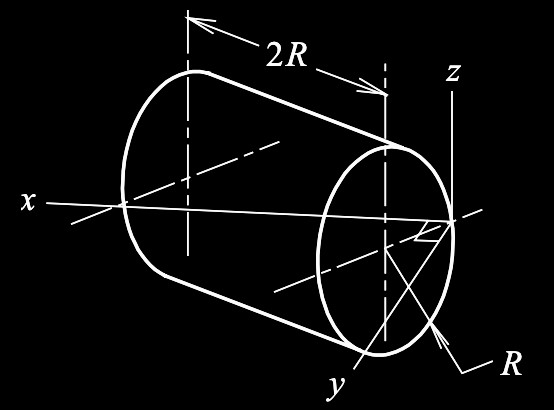
\includegraphics[scale=0.7,frame]{images/Q5_13.png}
% \end{figure}




\end{document}

